\documentclass{beamer}
\usepackage{textcomp}
\usepackage{graphicx}

\usetheme{Cuerna}

\author{Alireza Arzehgar}
\title{The Linux Community and a Career in Open Source}
\date{\today}

\newcommand{\copyleft}{\reflectbox{\copyright}}

\begin{document}
	\begin{frame}[plain]
		\maketitle
	\end{frame}

	\begin{frame}
		\frametitle{Introduction}
		\begin{itemize}
			\pause
			\item Linux Evolution and Popular Operating Systems
			\pause
			\item Major Open Source Applications
			\pause
			\item Open Source Software and Licensing 
			\pause
			\item ICT Skills and Working in Linux
		\end{itemize}
	\end{frame}

	\begin{frame}
		\frametitle{Linux Evolution and Popular Operating Systems}
		\begin{itemize}
			\pause
			\item Distributions
			\begin{itemize}
				\pause
				\item Debian, Ubuntu(LTS)
				\pause
				\item CentOS, openSUSE, Red Hat, SUSE
				\pause
				\item Linux Mint, Scientific Linux
				\pause
				\item Raspberry Pi, Raspbian
				\pause
				\item Android
			\end{itemize}
			\pause
			\item Embedded Systems
			\pause
			\item Linux in the Cloud
		\end{itemize}
	\end{frame}

	\begin{frame}
		\frametitle{GNU/Linux Desktops}
		\only{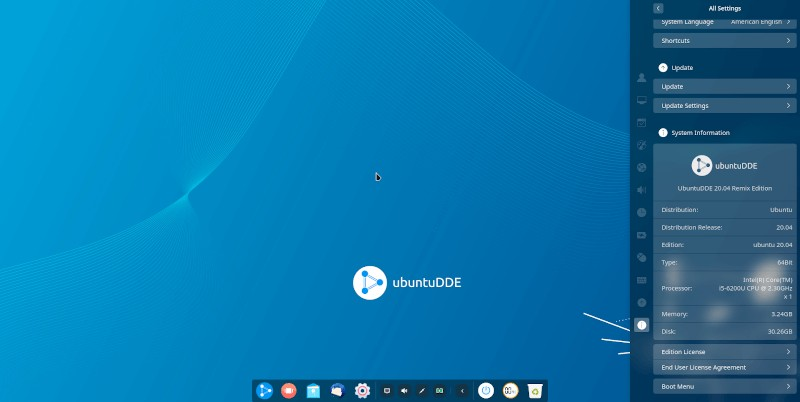
\includegraphics[width=\textwidth]{assets/deepin.jpg}}<1>
		\only{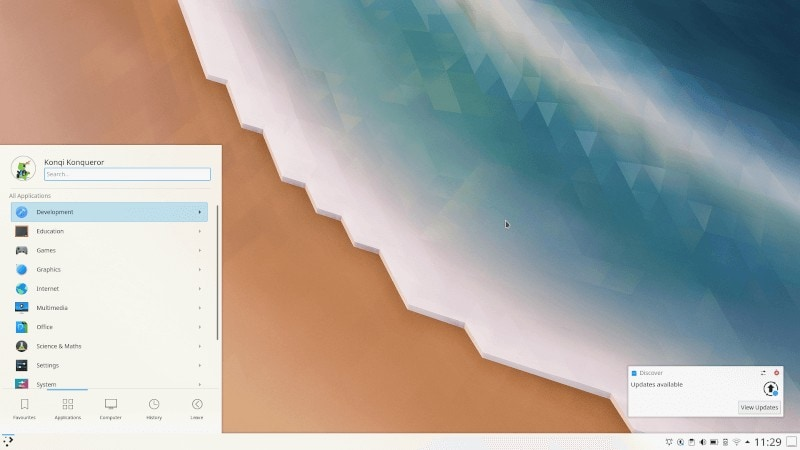
\includegraphics[width=\textwidth]{assets/kde.jpg}}<2>
		\only{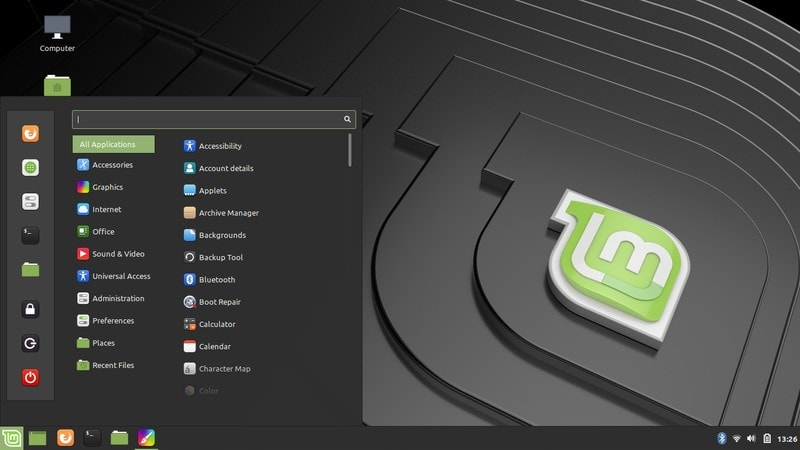
\includegraphics[width=\textwidth]{assets/mint.jpg}}<3>
		\only{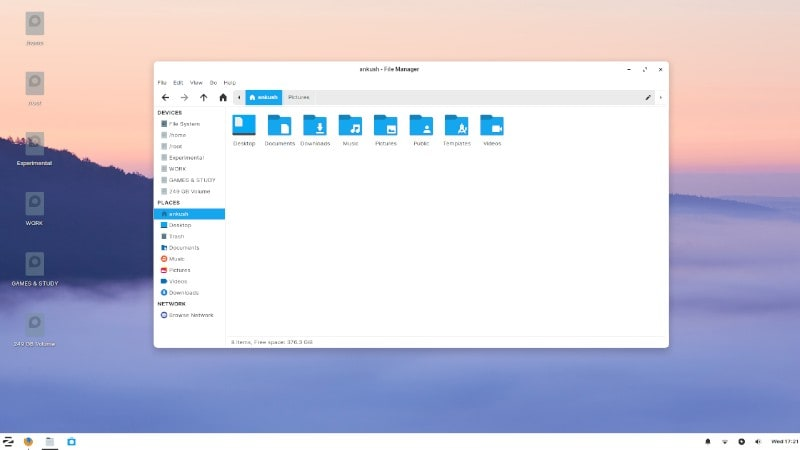
\includegraphics[width=\textwidth]{assets/xfce.jpg}}<4>
		\only{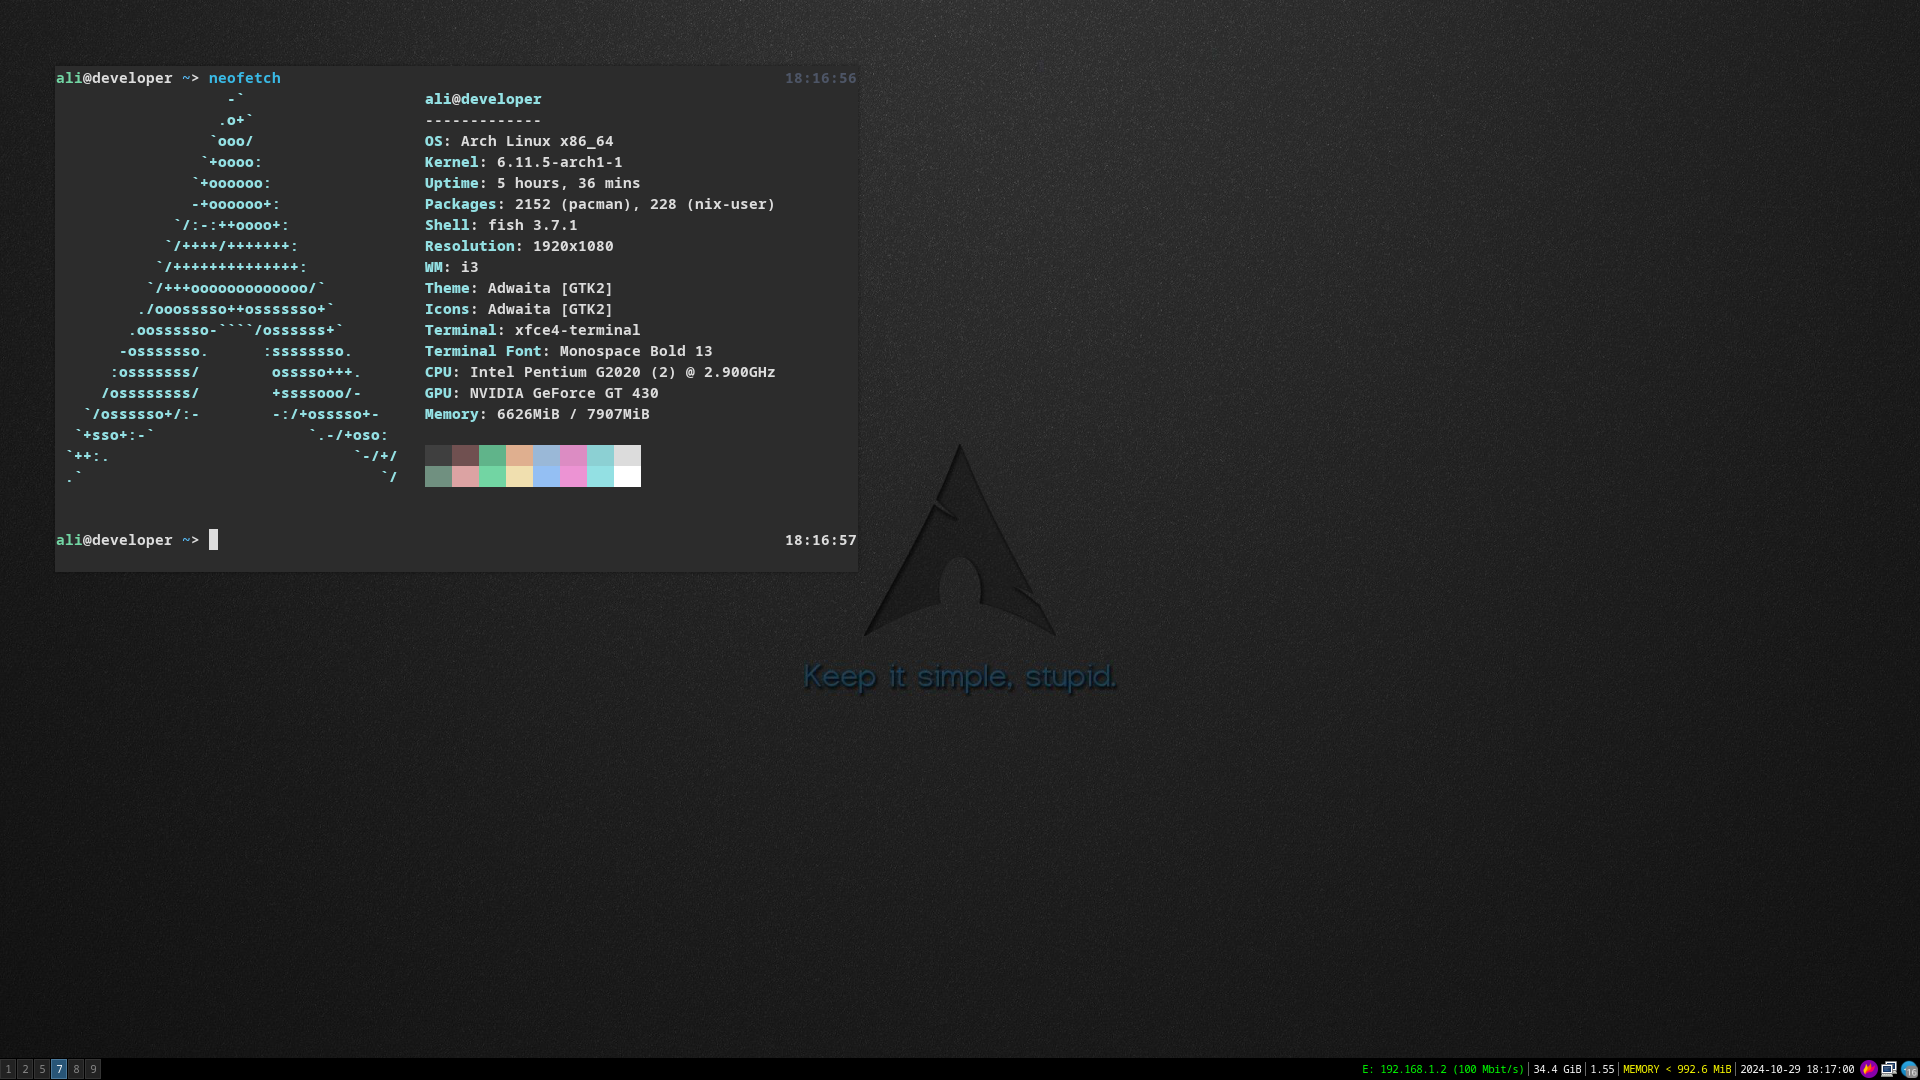
\includegraphics[width=\textwidth]{assets/me.jpg}}<5>
	\end{frame}

	\begin{frame}
		\frametitle{Major Open Source Applications}
		\begin{itemize}
			\pause
			\item Desktop applications
			\begin{itemize}
				\pause
				\item OpenOffice.org, LibreOffice, Thunderbird, Firefox, GIMP
			\end{itemize}

			\pause
			\item Server applications
			\begin{itemize}
				\pause
				\item Apache HTTPD, NGINX, MariaDB, MySQL, NFS, Samba
			\end{itemize}

			\pause
			\item Development languages
			\begin{itemize}
				\pause
				\item C, Java, JavaScript, Perl, shell, Python, PHP
			\end{itemize}

			\pause
			\item Package management tools and repositories
			\begin{itemize}
				\pause
				\item dpkg, apt-get, rpm, yum
			\end{itemize}
		\end{itemize}
	\end{frame}

	\begin{frame}
		\frametitle{Open Source Software and Licensing}
		\begin{itemize}
			\pause
			\item Open source philosophy
			\begin{itemize}
				\pause
				\item Copyleft \copyleft
				\pause
				\item Permissive
			\end{itemize}

			\pause
			\item Open source licensing
			\begin{itemize}
				\pause
				\item GPL
				\pause
				\item BSD
				\pause
				\item Creative Commons
			\end{itemize}

			\pause
			\item Free Software
			\begin{itemize}
				\pause
				\item Free Software Foundation (FSF)
				\pause
				\item Free Software
				\pause
				\item Open Source Software
				\pause
				\item FOSS
				\pause
				\item FLOSS
				\pause
				\item Open Source Initiative (OSI)
				\pause
				\item Open source business models
			\end{itemize}
		\end{itemize}
	\end{frame}

	\begin{frame}
		\frametitle{ICT Skills and Working in Linux}
		\begin{itemize}
			\pause
			\item Desktop skills
			\begin{itemize}
				\pause
				\item Using a browser, privacy concerns, configuration options, searching the web and saving content
			\end{itemize}

			\pause
			\item Getting to the command line
			\begin{itemize}
				\pause
				\item Password issues
				\pause
				\item Terminal and console
				\pause
				\item Privacy issues and tools
			\end{itemize}

			\pause
			\item Industry uses of Linux, cloud computing and virtualization
		\end{itemize}
	\end{frame}

\end{document}
